%! Author = angel

% Preamble
\documentclass[11pt]{article}

% Packages
\usepackage{amsmath,amssymb,amsthm}
\usepackage[letterpaper,margin=0.75in]{geometry}
\usepackage{pgfplots}
\usepackage{gensymb}
\usepackage{tikz}
\usepackage[usenames, dvipsnames]{xcolor}
\usepackage{fancyhdr}
\pgfplotsset{compat=1.18}
\usepackage{tikz-cd}
\usepackage{hyperref}
\colorlet{myblue}{black!40!blue}
\colorlet{myred}{black!40!red}
\tikzset{>=latex} % for LaTeX arrow head
\usetikzlibrary{decorations.markings, arrows.meta}
\usepackage{float}
% Document
\tikzset{
    marrow/.style={decoration={markings,mark=at position 0.5 with {\arrow{#1}}}, postaction=decorate}
}


\newcommand{\fahrenheit}{\degree \text{F}}

% Document
\begin{document}
    \noindent \textbf{Chapter 33: Electromagnetic Waves }% Document
    \vspace{1em}

    \noindent Electromagnetic waves consist of oscillating electric and magnetic fields.
    The electromagnetic wave travels perpendicular to the electric field $\vec{E} $, and magnetic field $\vec{B} $.
    We find magnitudes of the fields given by:
    \begin{equation}
        E = E_m \sin (kx - \omega t) \tag{electric field}
    \end{equation}
    \begin{equation}
        B = B_m \sin(kx - \omega t) \tag{magnetic field}
    \end{equation}
    \noindent These waves form a spectrum which include:
    \begin{center}
        Long waves, Radio waves, Infrared, visible light, Ultraviolet, X-rays and Gamma rays
    \end{center}
   In ascending order for frequency, and descending order for wavelength
    \\The speed of any electromagnetic wave in a vacuum is given by:
    \begin{equation}
        c = \frac{E}{B} = \frac{1}{\sqrt{\mu_0 \epsilon_0}} = 3.0 \times 10^8 \text{ m/s} \tag{speed of light}
    \end{equation}
    Where $\mu_0 = 4\pi \times 10^{-7}$ N/A$^2$.
    We find the rate of energy per unit area transported by the wave using the \textbf{Poynting vector } $\vec{S}$ (W/m$^2$):
    \begin{equation}
        \vec{S} = \frac{1}{\mu_0} \vec{E} \times \vec{B} \tag{Poynting vector}
    \end{equation}
    We can further rewrite this in terms solely as the electric field:
    \begin{equation}
      \hspace{3cm} S = \frac{1}{c \mu_0} E^2 \hspace{-1cm} \tag{instant energy flow rate}
    \end{equation}
    For finding the average power over time over a unit area, we find the intensity (W/m$^2$):
    \begin{equation}
        I = \frac{1}{c \mu_0} E_{rms}^2 \tag{intensity}
    \end{equation}
    Where $E_{rms} = \frac{E_m}{\sqrt{2}}$ is the root mean square,
    which is the average magnitude of the oscillating field.
    The energy of a light source radiates outwards as a sphere:
    \begin{equation}
      I = \frac{P_s}{4 \pi r^2} \tag{intensity}
    \end{equation}
    When a electromagnetic wave hits a surface, a force and pressure is applied to the surface,
    because these waves carry linear momentum.
    The momentum applied can either be fully absorbed by the surface:
    \begin{equation}
      \Delta p = \frac{\Delta U}{c} \tag{total absorption}
    \end{equation}
    causing the surface to gain energy from the radiation,
    or it can reflect off the surface:
    \begin{equation}
      \Delta p = \frac{2 \Delta U}{c} \tag{total reflection}
    \end{equation}
    in which the radiation is fully redirected to the path it was on.
    Finding the radiation pressure follows a similar process:
    \begin{equation}
      p_r = \frac{I}{c} \tag{total absorption}
    \end{equation}
    \begin{equation}
      p_r = \frac{2I}{c} \hspace{-6.4cm} \tag{total reflection back along the path} 
    \end{equation}
    Note that force can be found by multiplying the pressure by an area ($F = A \cdot p_r$).
    \newpage
    \noindent Since the electromagnetic wave always travels perpendicular to the electric and magnetic field,
    it can be modeled as as two perpendicular \textcolor{myblue}{electric} and \textcolor{myred}{magenetic} waves:
% Electromagnetic wave - colored
    \begin{figure}[H]
        \centering
        \begin{minipage}{0.56\textwidth}
            \centering
            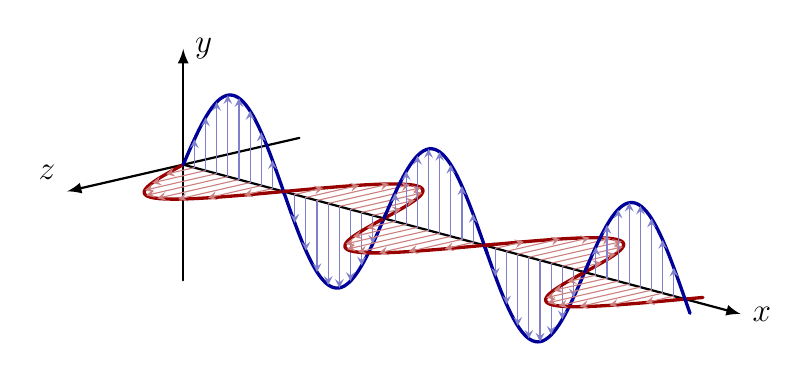
\begin{tikzpicture}[scale=0.7, x=(-15:1.2), y=(90:1.0), z=(-150:1.0),
                line cap=round, line join=round,
                axis/.style={black, thick,->},
                vector/.style={>=stealth,->}]
                \large
                \def\A{1.5}
                \def\nNodes{5} % use even number
                \def\nVectorsPerNode{8}
                \def\N{\nNodes*40}
                \def\xmax{\nNodes*pi/2*1.01}
                \pgfmathsetmacro\nVectors{(\nVectorsPerNode+1)*\nNodes}

                \def\drawENode{ % draw E node and vectors with some offset
                    \draw[myblue,very thick,variable=\t,domain=\iOffset*pi/2:(\iOffset+1)*pi/2*1.01,samples=40]
                    plot (\t,{\A*sin(\t*360/pi)},0);
                    \foreach \k [evaluate={\t=\k*pi/2/(\nVectorsPerNode+1);
                    \angle=\k*90/(\nVectorsPerNode+1);}]
                    in {1,...,\nVectorsPerNode}{
                        \draw[vector,myblue!50]  (\iOffset*pi/2+\t,0,0) -- ++(0,{\A*sin(2*\angle+\iOffset*180)},0);
                    }
                }
                \def\drawBNode{ % draw B node and vectors with some offset
                    \draw[myred,very thick,variable=\t,domain=\iOffset*pi/2:(\iOffset+1)*pi/2*1.01,samples=40]
                    plot (\t,0,{\A*sin(\t*360/pi)});
                    \foreach \k [evaluate={\t=\k*pi/2/(\nVectorsPerNode+1);
                    \angle=\k*90/(\nVectorsPerNode+1);}]
                    in {1,...,\nVectorsPerNode}{
                        \draw[vector,myred!50]  (\iOffset*pi/2+\t,0,0) -- ++(0,0,{\A*sin(2*\angle+\iOffset*180)});
                    }
                }

                % main axes
                \draw[axis] (0,0,0) -- ++(\xmax*1.1,0,0) node[right] {$x$};
                \draw[axis] (0,-\A*1.4,0) -- (0,\A*1.4,0) node[right] {$y$};
                \draw[axis] (0,0,-\A*1.4) -- (0,0,\A*1.4) node[above left] {$z$};

                % draw (anti-)nodes
                \foreach \iNode [evaluate={\iOffset=\iNode-1;}] in {1,...,\nNodes}{
                    \ifodd\iNode \drawBNode \drawENode % E overlaps B
                    \else        \drawENode \drawBNode % B overlaps E
                    \fi
                }

            \end{tikzpicture}
        \end{minipage}%
        \begin{minipage}{0.33\textwidth}
            \centering
            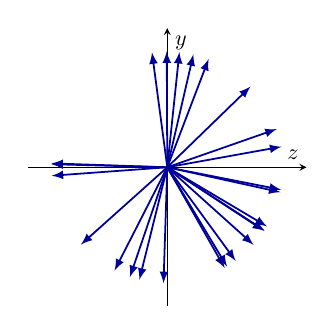
\begin{tikzpicture}[scale=0.8]
                \begin{axis}[
                axis lines=middle,
                enlargelimits=false,
                height=6cm,
                width=6cm,
                xmin=-1.2, xmax=1.2,
                ymin=-1.2, ymax=1.2,
                xtick=\empty, ytick=\empty,
                xlabel={$z$}, ylabel={$y$}
                ]

                % Number of vectors (adjust as needed)
                \foreach \i in {1,...,25} { % Adjust 25 for more or fewer vectors
                    \pgfmathsetmacro{\angle}{rand*360} % Generate a random angle
                    \pgfmathsetmacro{\x}{cos(\angle)}
                    \pgfmathsetmacro{\y}{sin(\angle)}
                    \addplot[->, thick, myblue] coordinates {(0,0) (\x,\y)};
                }

                \end{axis}
            \end{tikzpicture}
        \end{minipage}
    \end{figure}

    \noindent Most naturally occurring waves such as light do not always have perfectly defined electric and magnetic field orientations.
    Most waves from the front look like the right graph, where the fields are all oriented randomly.
    The orientation of the electric field is referred to as \textbf{polarization},
    in which the randomly polarized wave is considered unpolarized.
    \vspace{0.3cm}
    

 \begin{minipage}{0.25\textwidth}
\centering
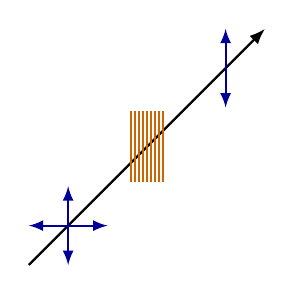
\begin{tikzpicture}[scale=0.5]

% Incident light ray (unpolarized)
\draw[black, thick, -{Latex[length=2mm]}] (-3,-3) -- (3,3);
% Polarizing sheet (circle with vertical lines)
\foreach \y in {-0.4,-0.3,...,0.4} {
  \draw[orange!80!black, thick] (\y,-0.9) -- (\y,0.9);
}

% Polarization symbols (unpolarized - cross)
\draw[myblue, thick, ->] (-2,-2) -- (-2,-1);
\draw[myblue, thick, ->] (-2,-2) -- (-2,-3);
\draw[myblue, thick, ->] (-2,-2) -- (-3,-2);
\draw[myblue, thick, ->] (-2,-2) -- (-1,-2);

% Polarized light symbol (vertical only)
\draw[myblue, thick, ->] (2,2)-- (2,3);
\draw[myblue, thick, ->] (2,2) -- (2,1);

\end{tikzpicture}
\end{minipage}
\hfill
\begin{minipage}{0.7\textwidth}
\vspace{0.1cm}
When unpolarized light passes through a polarizing sheet, only the component of the electric field aligned with the sheet’s transmission axis is allowed through. The result is linearly polarized light.
This causes for the intensity to drop by half, if the \textbf{incoming light is unpolarized:}
\begin{equation}
        I = \frac{1}{2} I_0 \tag{one-half rule}
        \end{equation}

\end{minipage}
\vspace{2em}

\noindent If the light is \textbf{already polarized,} and passes through another polarizing sheet,
    we must consider the polarization directions:
    \begin{equation}
        I = I_0 \cos^2(\theta_f - \theta_i ) \tag{cosine-squared rule}
    \end{equation}
Although light diffracts or spreads, we can aproximate the light's behavior as a straight ray.
We represent this beam of light as the incident ray with angle $\theta_1$.

\begin{minipage}{0.25\textwidth}
\begin{center}
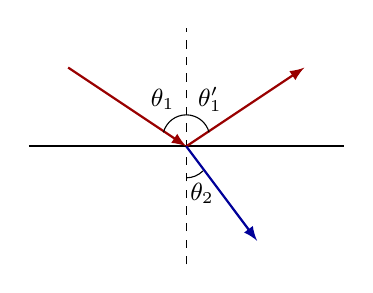
\begin{tikzpicture}[scale=1]

% Interface
\draw[thick] (-2,0) -- (2,0);

% Normal line
\draw[dashed] (0,-1.5) -- (0,1.5);

% Rays
\draw[->, thick, myred] (-1.5,1.0) -- (0,0);       % Incident ray
\draw[->, thick, myred] (0,0) -- (1.5,1.0);        % Reflected ray
\draw[->, thick, myblue] (0,0) -- (0.9,-1.2);       % Refracted ray

% Angle arcs (no labels)
\draw[-] (0,0.4) arc[start angle=90,end angle=15,radius=0.3];
\node at (0.3,0.6) {\small $\theta_1'$};  % Reflected angle label

\draw[-] (0,0.4) arc[start angle=90,end angle=165,radius=0.3];
\node at (-0.3,0.6) {\small $\theta_1$};  % Incident angle label

\draw[-] (0,-0.4) arc[start angle=270,end angle=315,radius=0.3];
\node at (0.2,-0.6) {\small $\theta_2$}; % Refracted angle label

\end{tikzpicture}

\end{center}

\end{minipage}
\hfill
\begin{minipage}{0.65\textwidth}
  \vspace{0.3cm}
  The incident ray can reflect off of a surface, redirecting its path resulting in \textbf{reflection:}
\begin{equation}
  \theta_1 = \theta_1 ' \tag{reflection}
\end{equation}
However, the beam of light can through a surface such as glass, forming a new angle, known as \textbf{refraction:}
\begin{equation}
  n_1 \sin \theta_1 = n_2 \sin \theta_2 \tag{Snell's Law}
\end{equation}
\end{minipage}
\vspace{1em}

\noindent The values $n$ are the index of refraction which refers to how much a medium slows down light,
giving the equation $n = c /v$ where $c$ is the speed of light in the medium.

\vspace{1em} 
\noindent Depending on the angle that the incident ray hits a surface, the refraction angle will be 90\degree,
meaning that no light passed through, and all of the light reflected back.
Total internal reflection occurs for all angles equal to greater than the \textbf{critical angle:}
\begin{equation}
  \theta_c = \sin^{-1}(\frac{n_2}{n_1}) \tag{critical angle}
\end{equation}

\noindent If an unpolarized light hits a surface at the \textbf{Brewster angle} $\theta_B$,
the reflected light will be fully polarized, and the refracted ray will be partially polarized.
\begin{equation}
\theta_B = \tan^{-1}(\frac{n_2}{n_1}) \tag{Brewster angle}
\end{equation}
\end{document}


